\documentclass[aspectratio=169]{beamer}
%\usetheme{CambridgeUS}
%\usecolortheme{beaver}

%\usefonttheme{serif}
%\usepackage{helvet}

\usefonttheme{serif}     % Font theme: serif
%\usepackage{ccfonts}     % Font family: Concrete Math
\usepackage[T1]{fontenc} % Font encoding: T1

\setbeamersize{text margin left=42pt,text margin right=42pt} 
\setbeamertemplate{navigation symbols}{}
\setbeamertemplate{itemize items}[default]

\beamertemplatenavigationsymbolsempty

\definecolor{fore}{RGB}{51,51,51}
\definecolor{back}{RGB}{255, 254, 250}
\definecolor{title}{RGB}{ 255, 15, 0}
\definecolor{links}{RGB}{18, 168, 255}

\setbeamercolor{titlelike}{fg=title}
\setbeamercolor{normal text}{fg=fore,bg=back}
\setbeamercolor{alerted text}{fg=title}
\setbeamercolor{itemize item}{fg=title}
\setbeamercolor{enumerate item}{fg=title}
\hypersetup{colorlinks,urlcolor=links}

% for code https://kbroman.org/blog/2013/10/07/better-looking-latexbeamer-slides/
\usepackage{listings}
\definecolor{keywords}{RGB}{255,0,90}
\definecolor{comments}{RGB}{60,179,113}
\lstset{language=Python,
keywordstyle=color{keywords},
commentstyle=color{comments}emph}

% fonts
\usepackage[sc]{mathpazo}


% title info
\title{\textbf{Course Introduction}}
\subtitle{\textbf{GGR424 - Transportation Geography \& Planning}}
\author{Jeff Allen}
\institute{University of Toronto}
\date{January 10, 2022}


\begin{document}
	
\begin{frame}
	\titlepage	
\end{frame}



\begin{frame}
\textbf{Today:}
\begin{itemize}
	\item Introductions
	\item Why study transportation?
	\item Course Outline
	\item Core Concepts
	\item Mode prioritization
\end{itemize}
\end{frame}




\begin{frame}
\LARGE{\textbf{Introductions:}}
\end{frame}

\begin{frame}
\textbf{About Me}
\begin{itemize}
	\item PhD Candidate in Geography
	\item Researches Urban Geography/Planning, Transportation, \& GIS
	\item Cartography / Data Science Consulting
\end{itemize}
\end{frame}





\begin{frame}
	\LARGE{\textbf{Why Study Transportation?}}
\end{frame}



\begin{frame}
	\textbf{Why Study Transportation? Injuries and Death}
	\begin{figure}
		\centering
		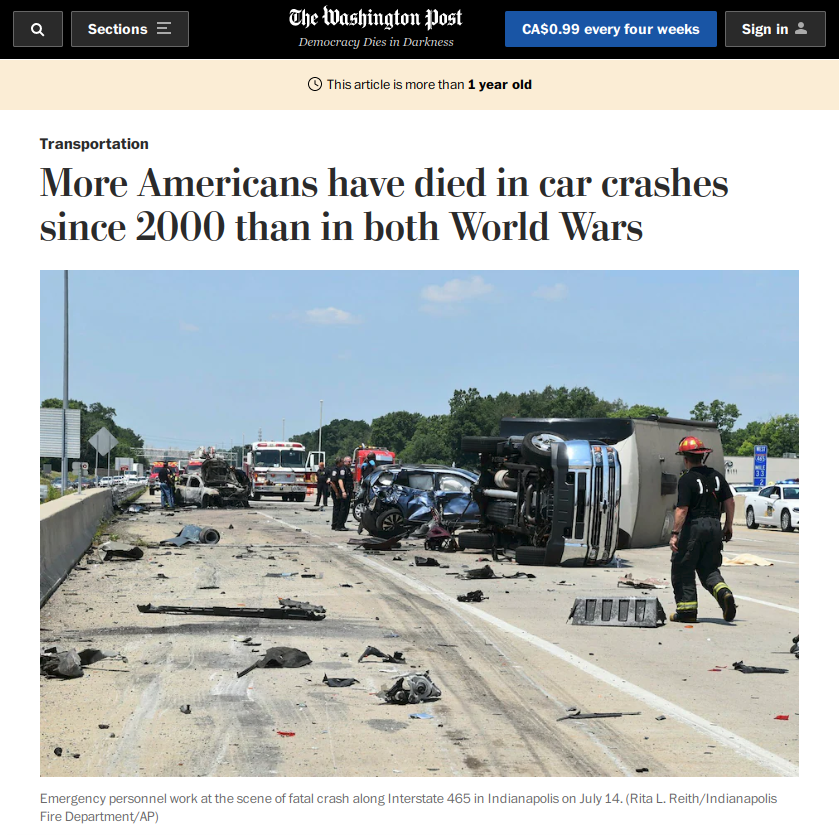
\includegraphics[width=0.5\linewidth]{images/wash_post_deaths.png}
	\end{figure}
	\tiny\url{https://www.washingtonpost.com/local/trafficandcommuting/more-people-died-in-car-crashes-this-century-than-in-both-world-wars/2019/07/21/0ecc0006-3f54-11e9-9361-301ffb5bd5e6_story.html}
\end{frame}


\begin{frame}
	\textbf{Why Study Transportation? Injuries and Death}
	\begin{figure}
		\centering
		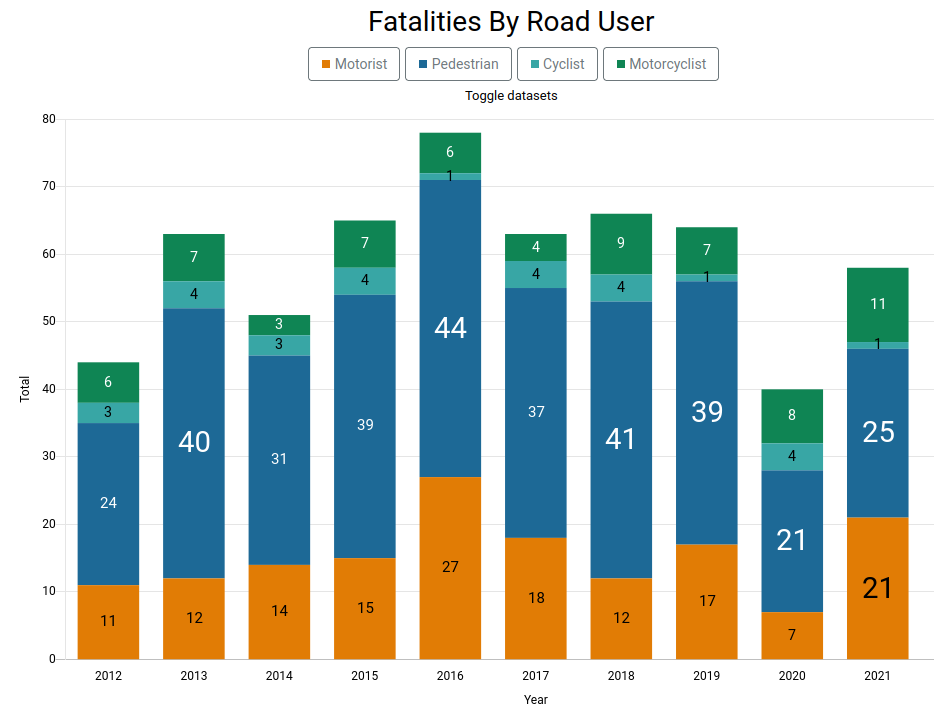
\includegraphics[width=0.7\linewidth]{images/vision_zero_deaths.png}
	\end{figure}
	\tiny\url{https://www.toronto.ca/services-payments/streets-parking-transportation/road-safety/vision-zero/vision-zero-dashboard/fatalities-vision-zero/}
\end{frame}
% when did vision zero start?
% traffic in fatalities in Canada have been decreasing - safer cars and roads? - but less so in our cities, more congestion?
% https://tc.canada.ca/en/road-transportation/statistics-data/canadian-motor-vehicle-traffic-collision-statistics-2019




\begin{frame}
	\textbf{Why Study Transportation? Environment}
	\begin{figure}
		\centering
		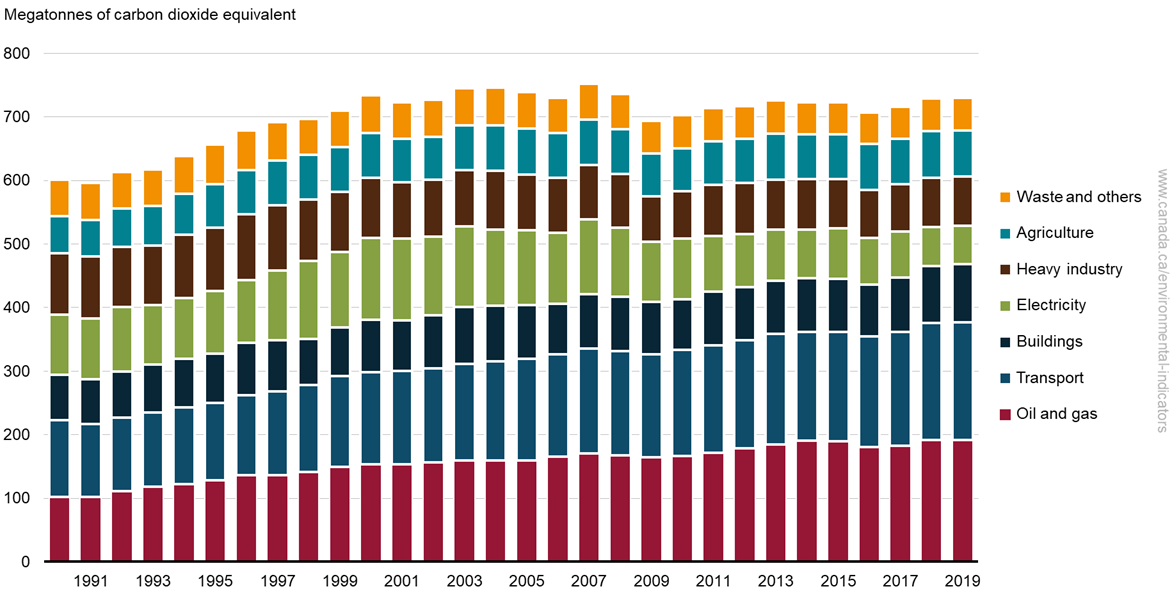
\includegraphics[width=0.8\linewidth]{images/canada_emissions_by_sector.png}
	\end{figure}
\end{frame}


\begin{frame}
	\textbf{Why Study Transportation? Environment}
	\begin{figure}
		\centering
		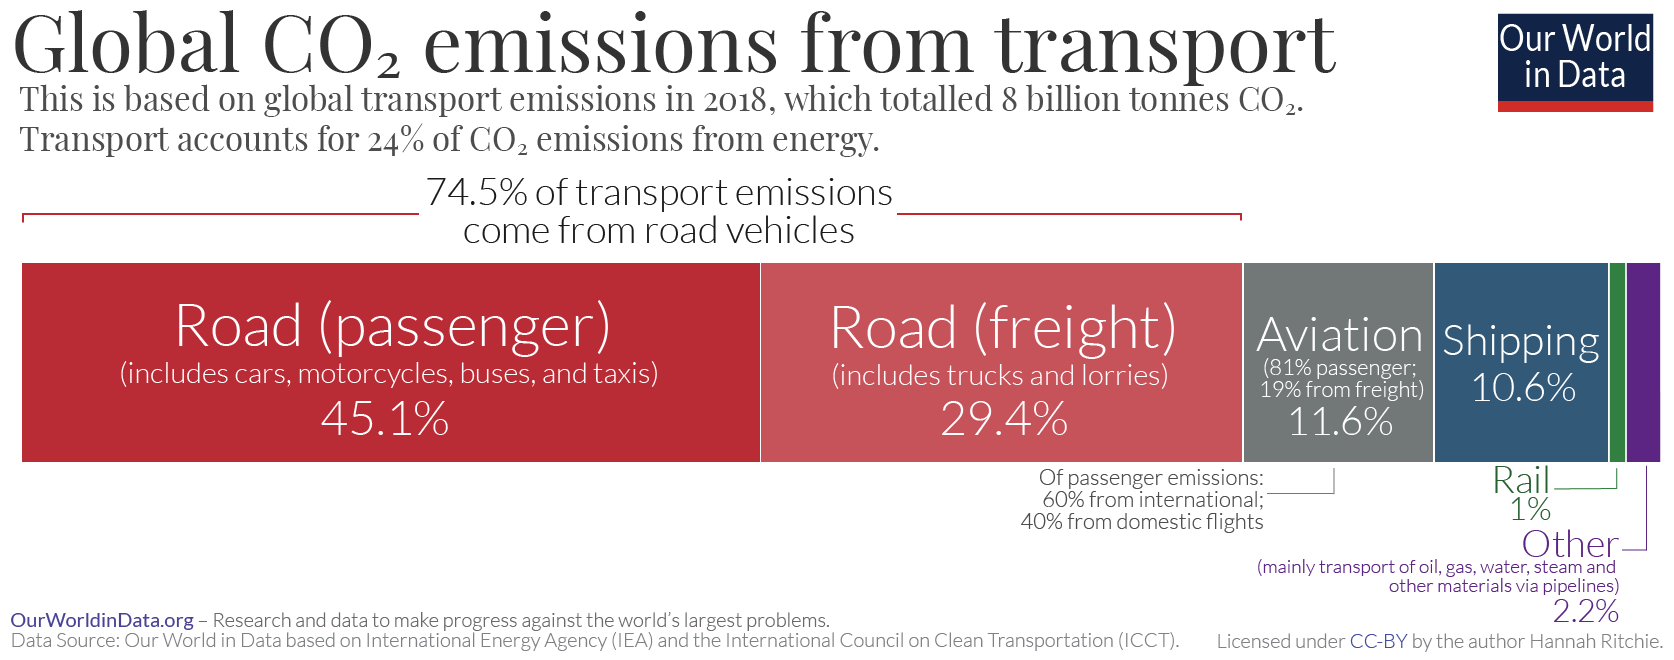
\includegraphics[width=0.8\linewidth]{images/Transport-CO2-emissions-by-mode-bar-chart.png}
	\end{figure}
\end{frame}




\begin{frame}
	\textbf{Why Study Transportation? Congestion}
	\begin{figure}
		\centering
		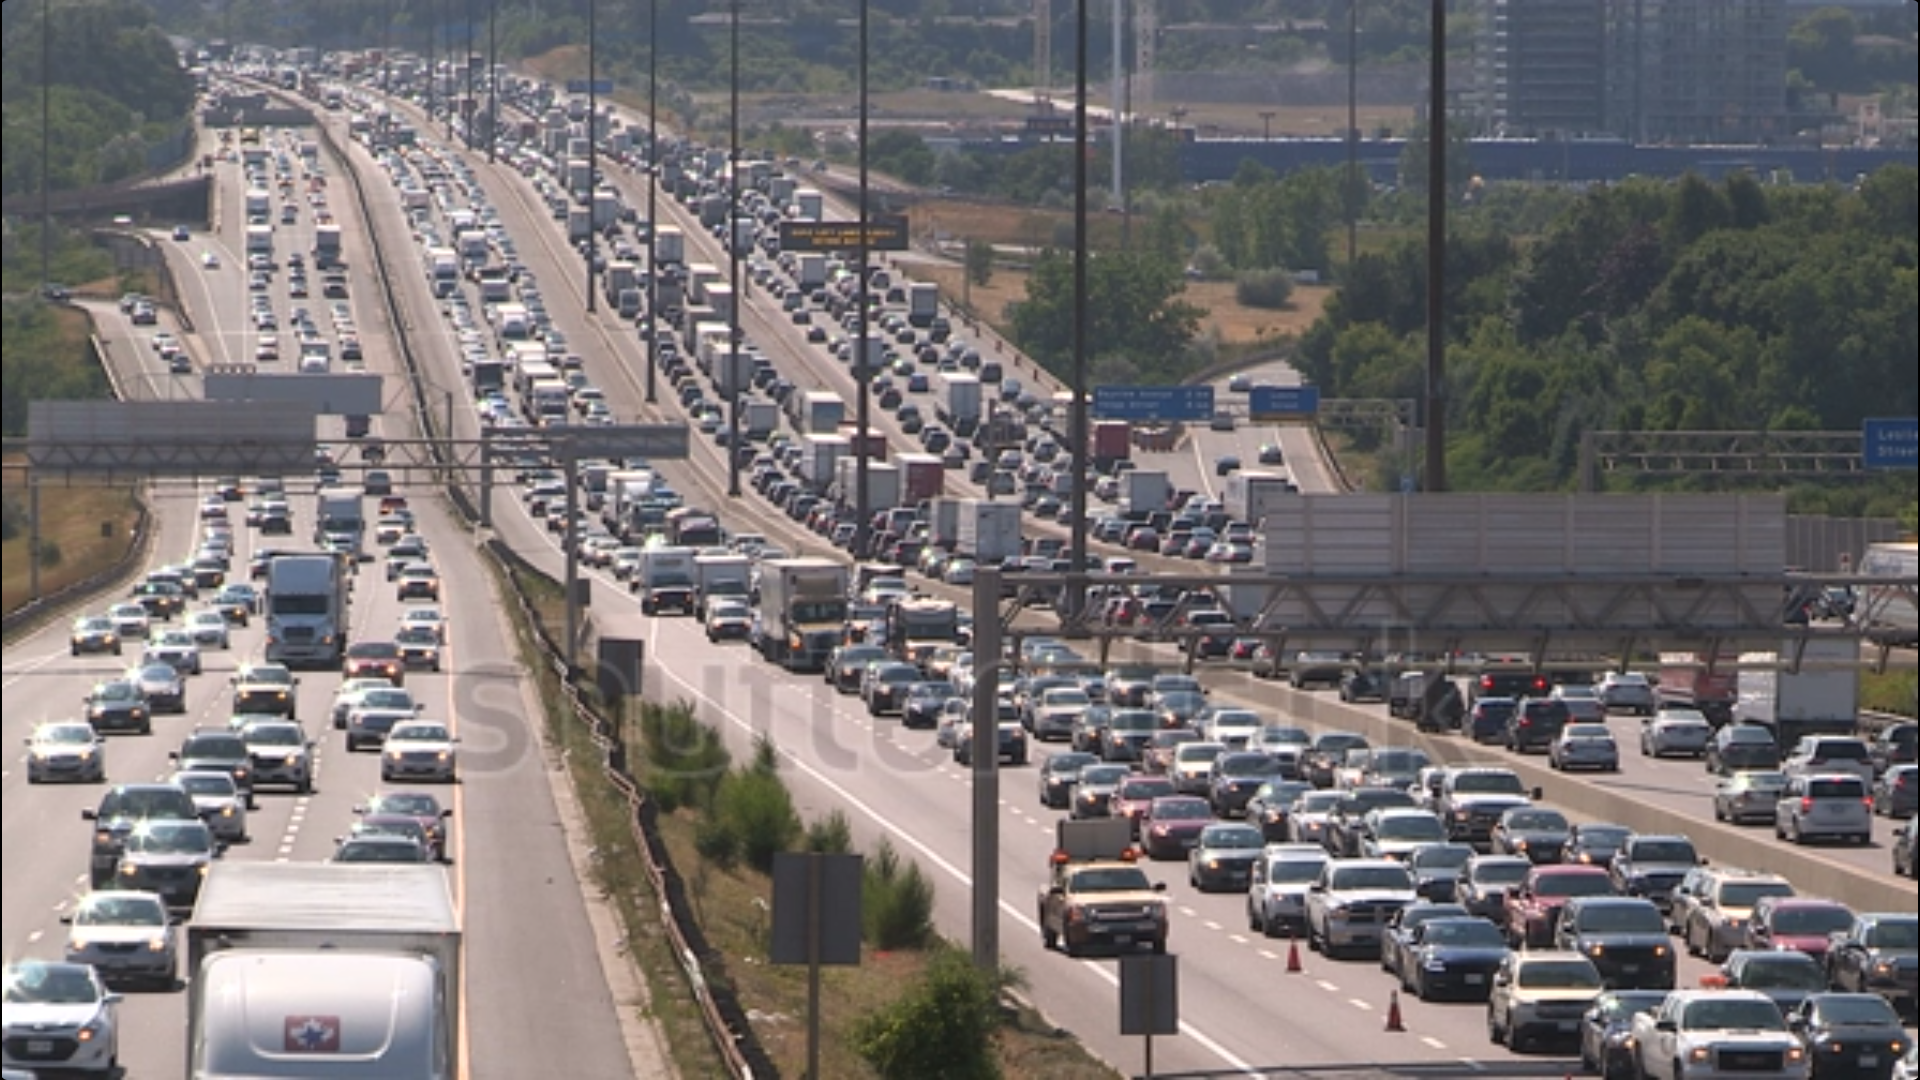
\includegraphics[width=0.8\linewidth]{images/traffic_401.png}
	\end{figure}
	\tiny\url{https://www.shutterstock.com/video/clip-18150214-toronto-ontario-canada-july-2015-epic-rush}
\end{frame}
% pollution
% impacts both on health and environment


\begin{frame}
	\textbf{Why Study Transportation? Congestion}
	\begin{figure}
		\centering
		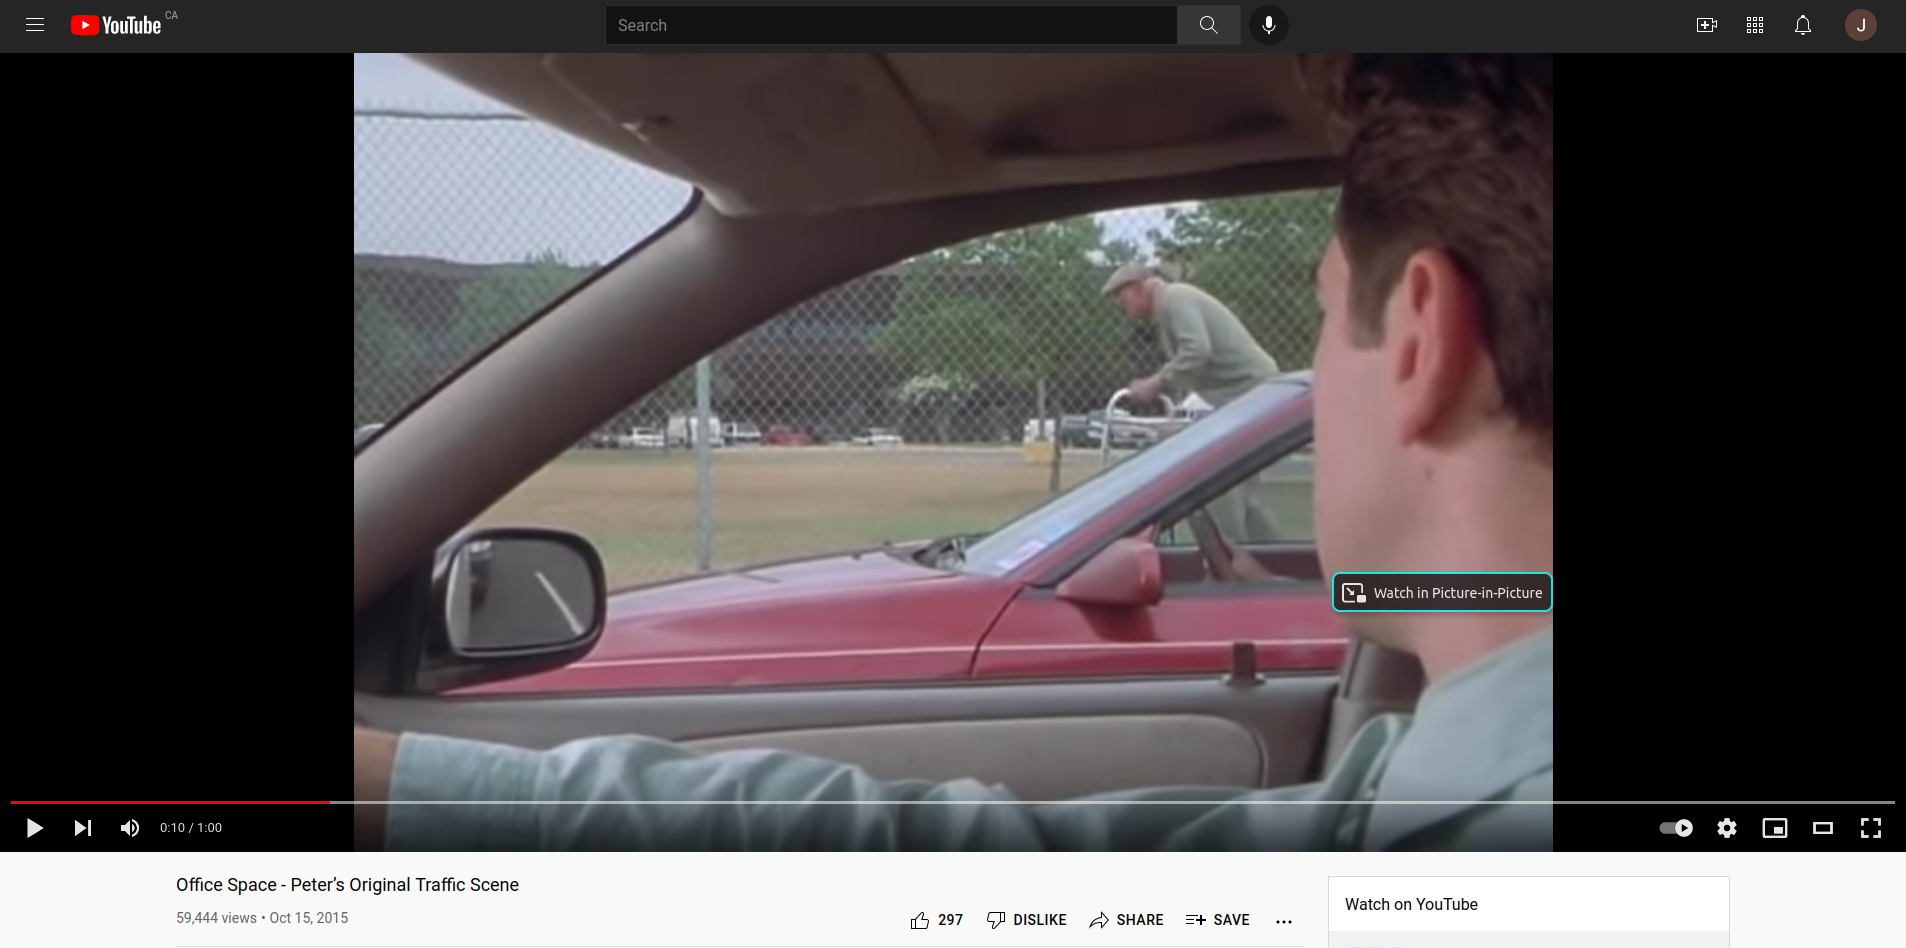
\includegraphics[width=0.8\linewidth]{images/office_space.png}
	\end{figure}
	\tiny\url{https://www.youtube.com/watch?v=LcCdB46MybQ}
\end{frame}

% https://toronto.ctvnews.ca/drivers-in-toronto-lose-142-hours-on-the-roads-during-rush-hour-report-finds-1.4790478


% wasted time, car based life styles bad for health



\begin{frame}
	\textbf{Why Study Transportation? Land Use}
	\begin{figure}
		\centering
		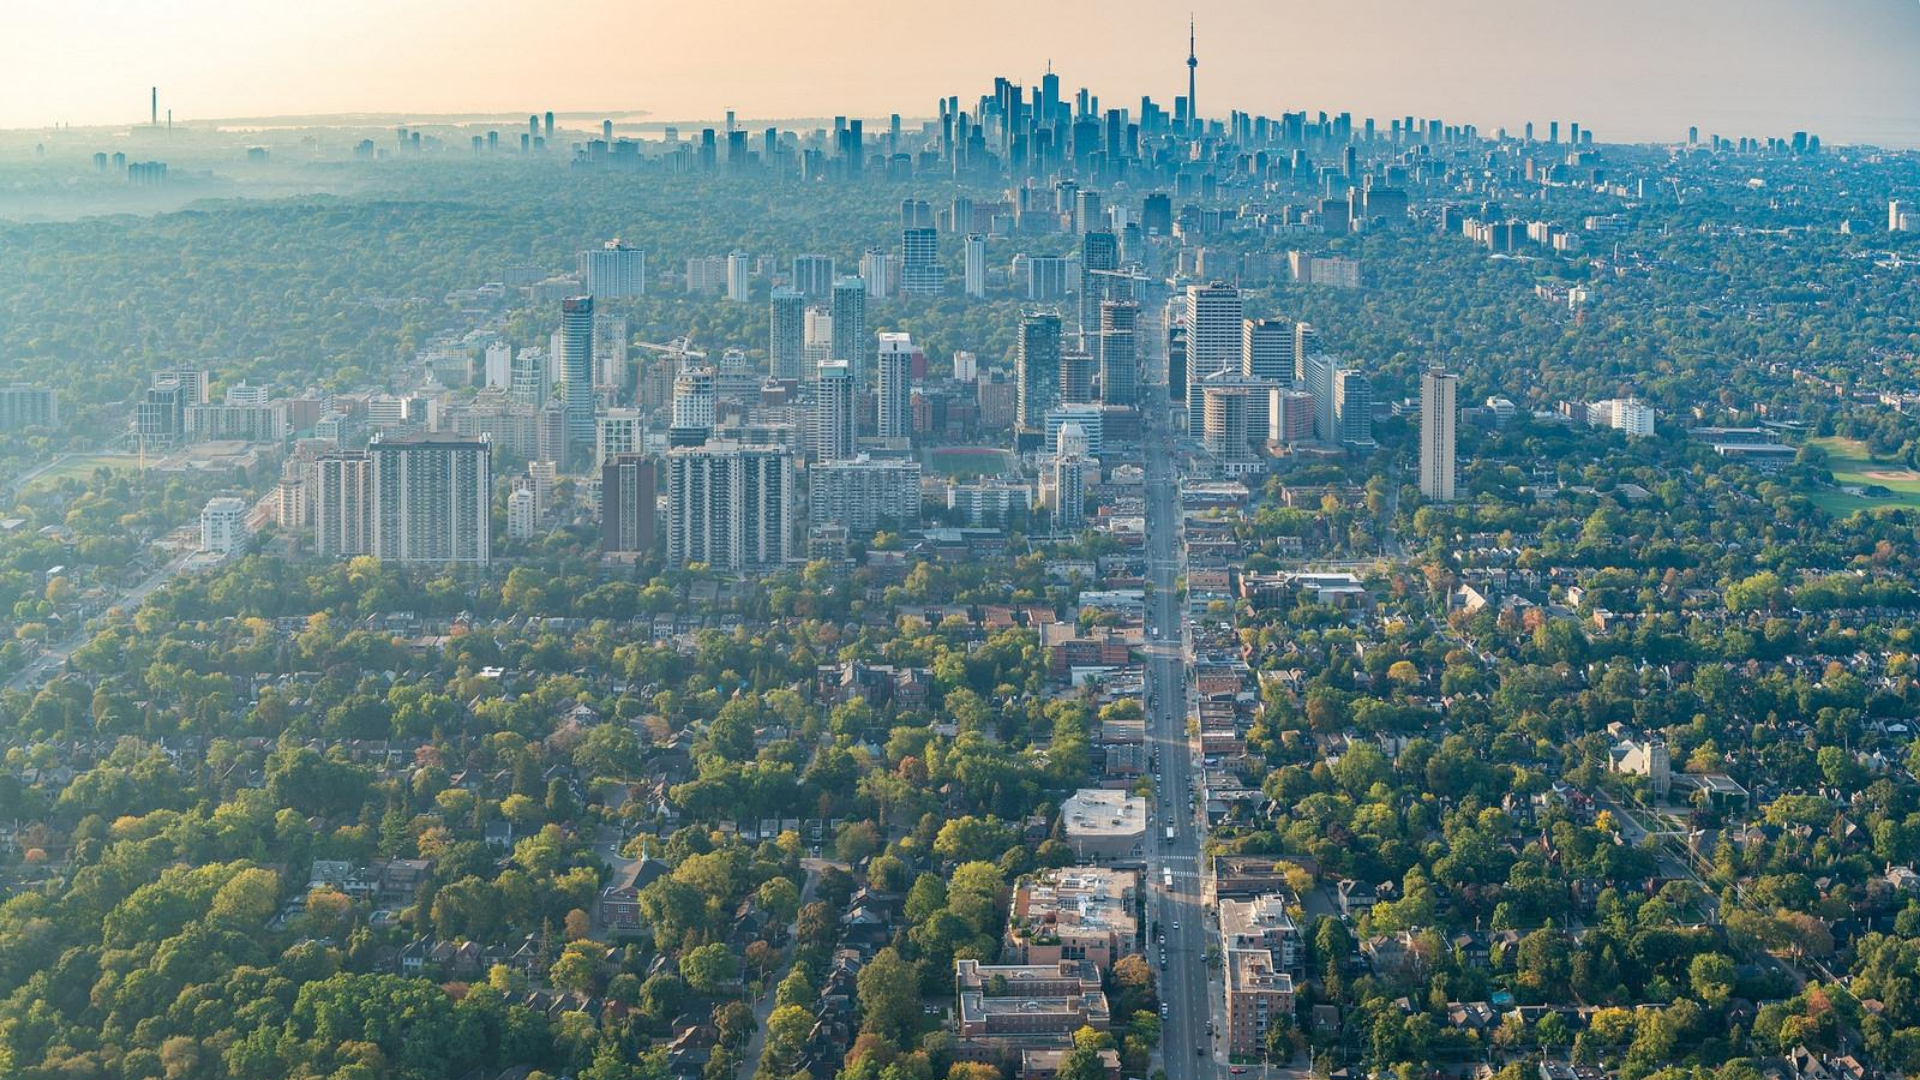
\includegraphics[width=0.9\linewidth]{images/i3.png}
	\end{figure}
\end{frame}

\begin{frame}
	\textbf{Why Study Transportation? Land Use}
	\begin{figure}
		\centering
		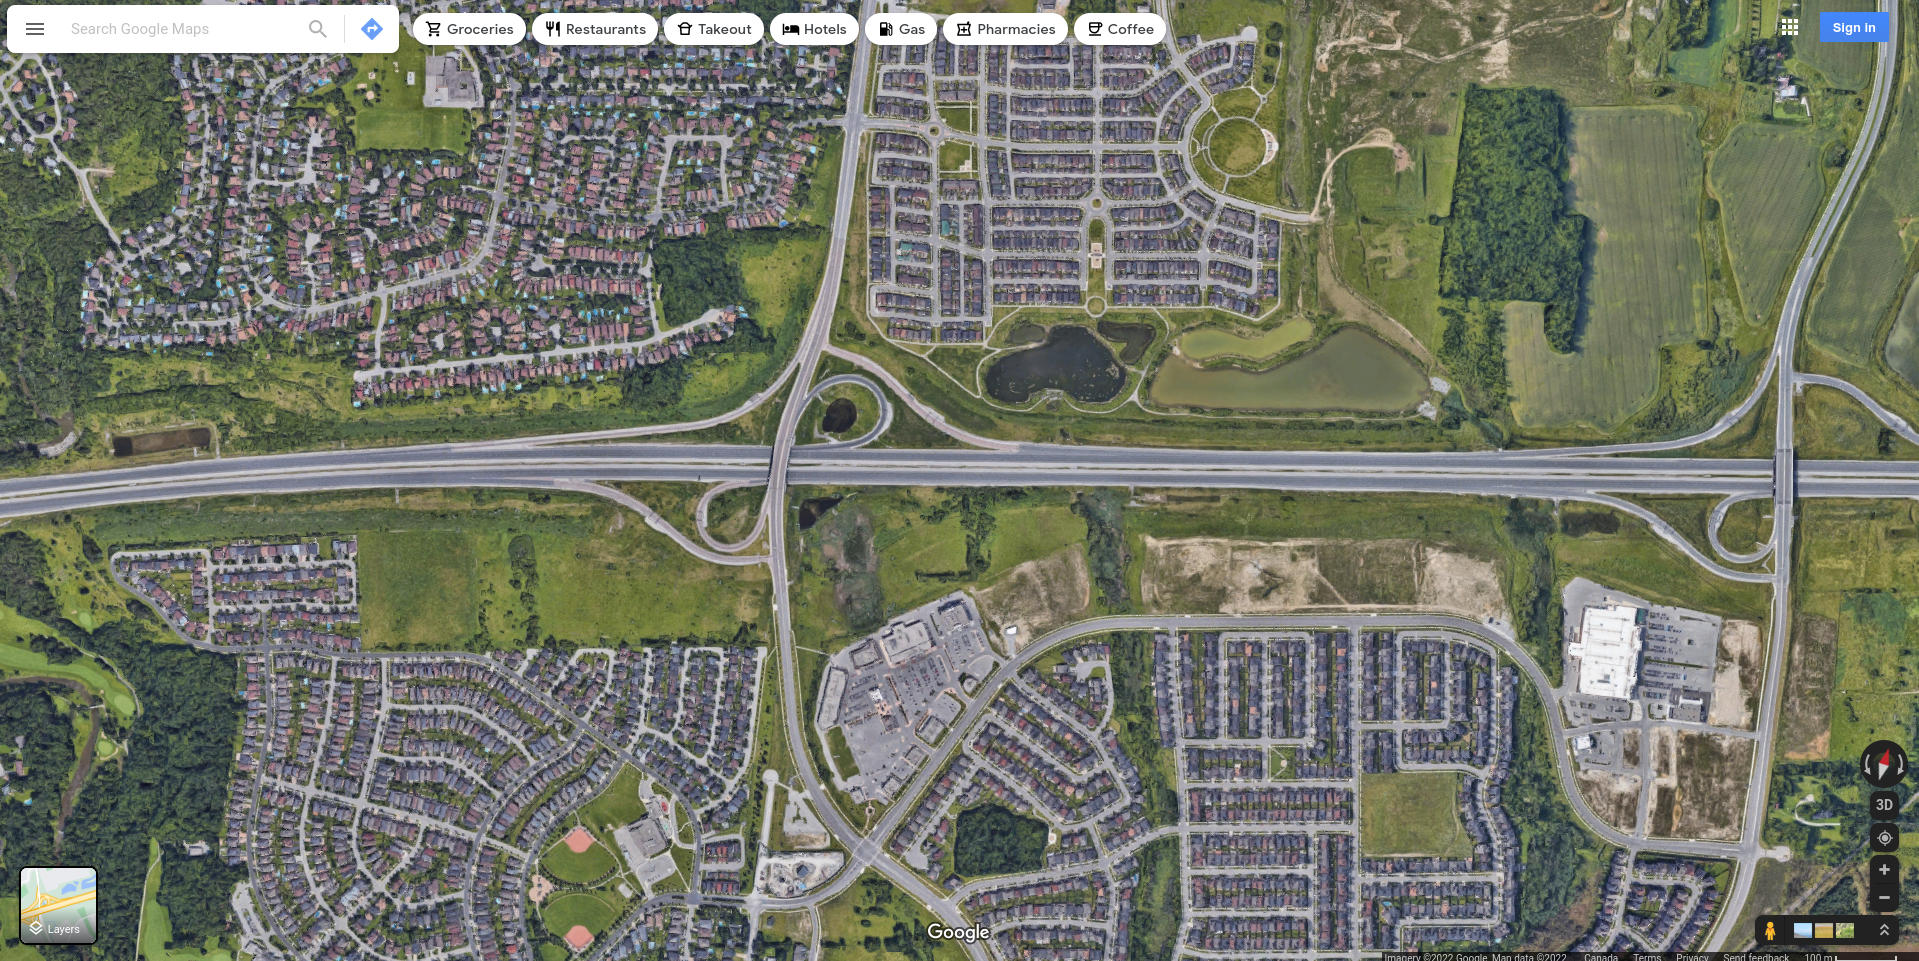
\includegraphics[width=0.9\linewidth]{images/sprawl_markham407.png}
	\end{figure}
\end{frame}


\begin{frame}
	\textbf{Why Study Transportation? Land Use}
	\begin{figure}
		\centering
		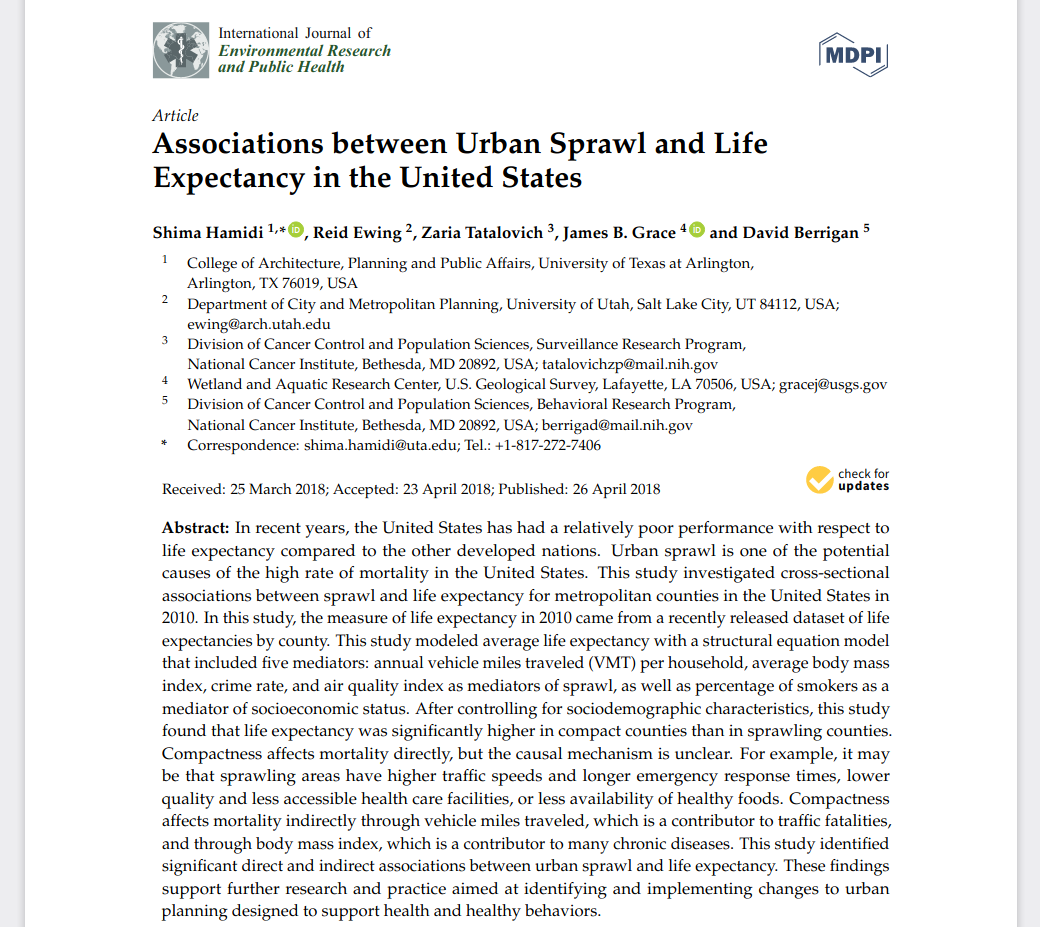
\includegraphics[width=0.6\linewidth]{images/sprawl_life_expectancy.png}
	\end{figure}
\end{frame}


\begin{frame}
	\textbf{Why Study Transportation? Inequality}
	\begin{figure}
		\centering
		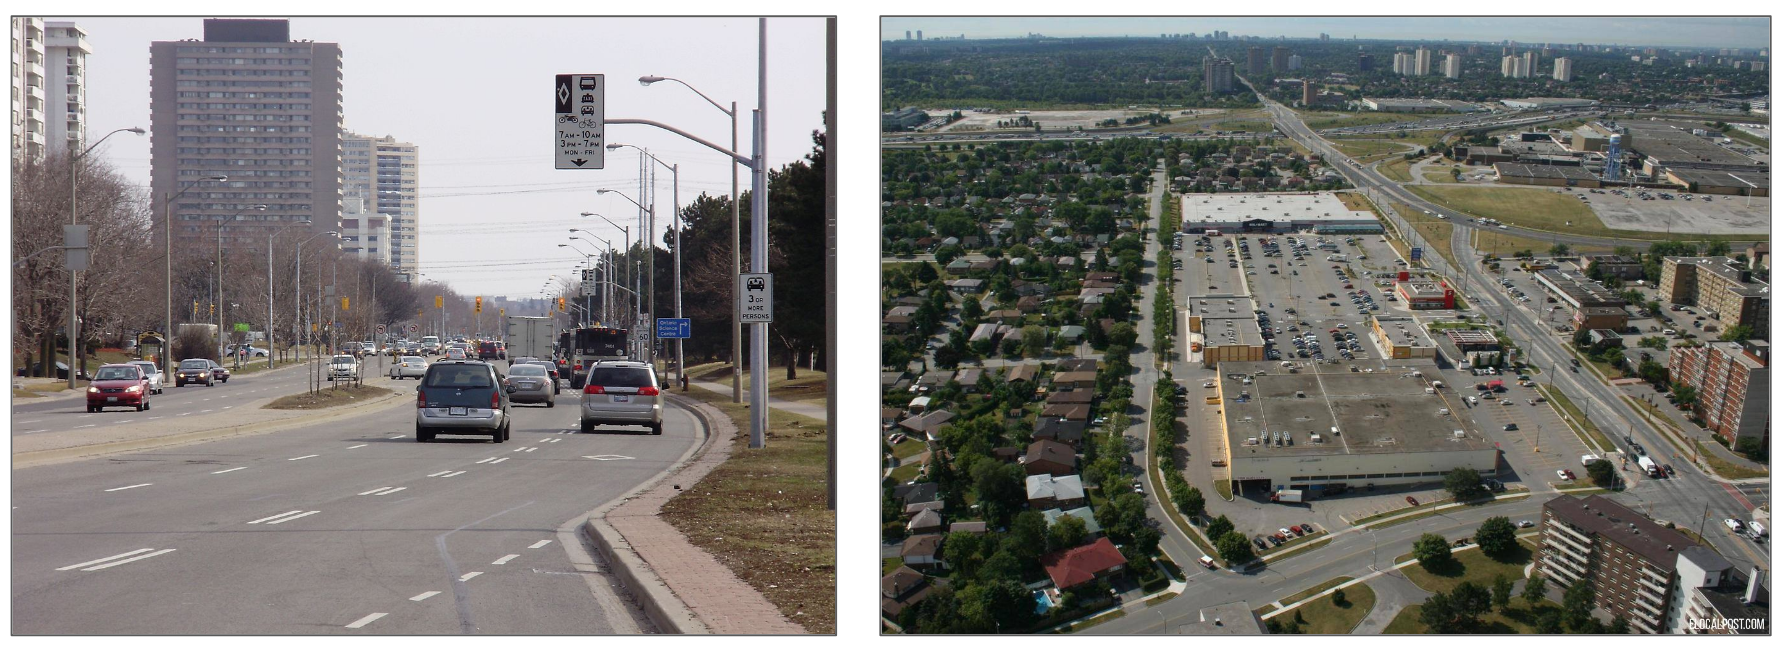
\includegraphics[width=1\linewidth]{images/suburbs_tor.png}
	\end{figure}
\end{frame}


\begin{frame}
	\textbf{Why Study Transportation? Inequality}
	\begin{figure}
		\centering
		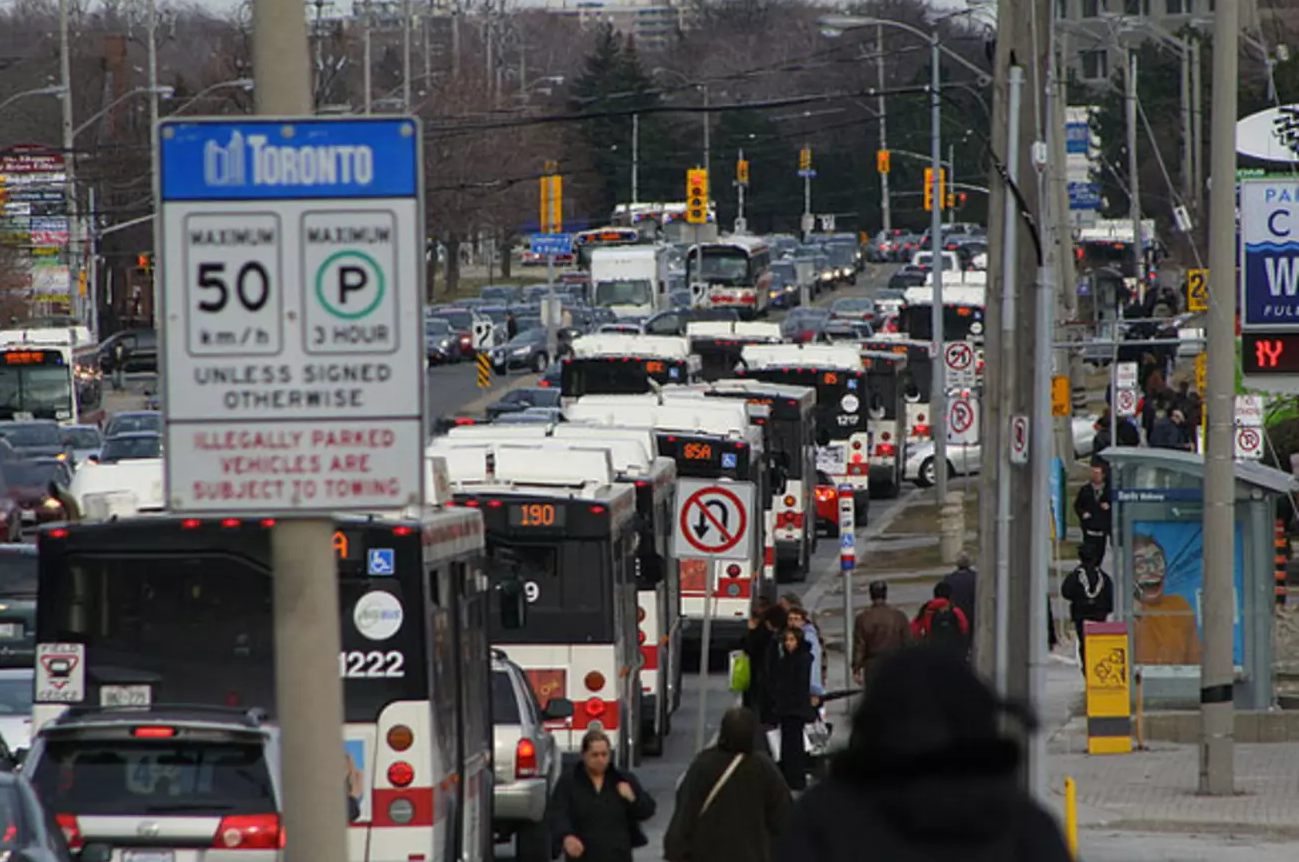
\includegraphics[width=0.8\linewidth]{images/ttc_traffic.png}
	\end{figure}
\end{frame}


% not all doom and gloom

\begin{frame}
	\textbf{Why Study Transportation? Benefits!}
	\begin{figure}
		\centering
		\includegraphics[width=0.7\linewidth]{images/utrecht1.jpg}
	\end{figure}
	\tiny\url{https://en.wikipedia.org/wiki/Utrecht}
\end{frame}

% get to destinations
% walkability
% some commutes enjoyable



\begin{frame}

\textbf{Course Objectives}
		\small
		\begin{itemize}
			\item Understand fundamental concepts and theories in urban transportation geography and planning.
			
			\item Identify and critically assess major social, political, economic, and environmental issues related to urban transportation.
			
			\item Analyze and visualize transportation-related data (including using GIS) to describe travel behaviour, transportation networks, land use, and accessibility.
			
			\item Apply the theoretical and practical knowledge you have acquired from the course to develop recommendations on improving urban transport systems.
		\end{itemize}

\end{frame}





\begin{frame}
	\LARGE{\textbf{Course Outline}}
	
	\vspace{4mm}
	
	\small
	\textit{(open up the syllabus)}
\end{frame}

% TALK ABOUT A1!




\begin{frame}
	\LARGE{\textbf{Key Concepts in Urban Transportation}}
	\normalsize
	\vspace{4mm}
	\begin{itemize}
		\item Demand
		\item Activity Participation
		\item Utility
		\item Transport \& Land Use
		\item Travel Behaviour
		% \item Mobility VS Accessibility
	\end{itemize}
\end{frame}


	% Overview of what?
% system approach, 
% transport networks and land use
% social, env, econmoic impacts
% travel behaviour / trips

% concepts:

% utility
% demand
% mobility vs accessibility

% see SF slides 2

% transportationi is a complex system
% networks > land use > travel behaviour 

% networks slide

% land use slide

% trips slide

% what arer the qualities a trip?
% time, distance, mode, purpose
% subjective, satisfaction, etc.
% 




\begin{frame}
	\textbf{Next Week} 
	
	\vspace{4mm}
	
	Cars, Roads, \& Highways:
	
	\begin{itemize}
		
		% \item Mobility VS Accessibility
		
		\item Rise of cars as the predominant mode of travel in Canadian cities. 
		
		\item How the infrastructure of automobiles has transformed transportation and land-use and has affected daily life. 
	\end{itemize}

\end{frame}



\end{document}